\documentclass[t]{beamer}
%\documentclass[finnish,english,handout]{beamer}

% Uncomment if want to show notes
% \setbeameroption{show notes}

\mode<presentation>
{
  \usetheme{Copenhagen}
  % oder ...
  
  %\setbeamercovered{transparent}
  % oder auch nicht
}


\usepackage[T1]{fontenc}
\usepackage[latin1]{inputenc}
\usepackage{times}
\usepackage{epic,epsfig}
\usepackage{subfigure,float}
\usepackage{amsmath,amsfonts,amssymb}
\usepackage{inputenc}
\usepackage{afterpage}
\usepackage{url}
\urlstyle{same}
\usepackage{amsbsy}
\usepackage{eucal}
\usepackage{rotating}
\usepackage{listings}
\usepackage{lstbayes}
\usepackage[all,poly,ps,color]{xy}
\usepackage{eurosym}
\usepackage{microtype}

\usepackage{natbib}
\bibliographystyle{apalike}

\hypersetup{%
  bookmarksopen=true,
  bookmarksnumbered=true,
  pdftitle={Stan},
  pdfsubject={Bayesian data analysis},
  pdfauthor={Aki Vehtari},
  pdfkeywords={},
  pdfstartview={FitH -32768},
  colorlinks=true,
  linkcolor=navyblue,
  citecolor=navyblue,
  filecolor=navyblue,
  urlcolor=navyblue
}

% \definecolor{hutblue}{rgb}{0,0.2549,0.6784}
% \definecolor{midnightblue}{rgb}{0.0977,0.0977,0.4375}
% \definecolor{hutsilver}{rgb}{0.4863,0.4784,0.4784}
% \definecolor{lightgray}{rgb}{0.95,0.95,0.95}
% \definecolor{section}{rgb}{0,0.2549,0.6784}
% \definecolor{list1}{rgb}{0,0.2549,0.6784}
\definecolor{forestgreen}{rgb}{0.1333,0.5451,0.1333}
\definecolor{navyblue}{rgb}{0,0,0.5}
\renewcommand{\emph}[1]{\textcolor{navyblue}{#1}}

\graphicspath{{./figs/}}

\pdfinfo{            
  /Title      (Bayesian data analysis 4)
  /Author     (Aki Vehtari) % 
  /Keywords   (Bayesian probability theory, Bayesian inference, Bayesian data analysis)
}


\parindent=0pt
\parskip=8pt
\tolerance=9000
\abovedisplayshortskip=0pt

\setbeamertemplate{navigation symbols}{}
\setbeamertemplate{headline}[default]{}
\setbeamertemplate{headline}[text line]{\insertsection}
\setbeamertemplate{footline}[frame number]


\def\o{{\mathbf o}}
\def\t{{\mathbf \theta}}
\def\w{{\mathbf w}}
\def\x{{\mathbf x}}
\def\y{{\mathbf y}}
\def\z{{\mathbf z}}

\DeclareMathOperator{\E}{E}
\DeclareMathOperator{\Var}{Var}
\DeclareMathOperator{\var}{var}
\DeclareMathOperator{\Sd}{Sd}
\DeclareMathOperator{\sd}{sd}
\DeclareMathOperator{\Gammad}{Gamma}
\DeclareMathOperator{\Invgamma}{Inv-gamma}
\DeclareMathOperator{\Bin}{Bin}
\DeclareMathOperator{\Negbin}{Neg-bin}
\DeclareMathOperator{\Poisson}{Poisson}
\DeclareMathOperator{\Beta}{Beta}
\DeclareMathOperator{\logit}{logit}
\DeclareMathOperator{\N}{N}
\DeclareMathOperator{\U}{U}
\DeclareMathOperator{\BF}{BF}
\DeclareMathOperator{\Invchi2}{Inv-\chi^2}
\DeclareMathOperator{\NInvchi2}{N-Inv-\chi^2}
\DeclareMathOperator{\InvWishart}{Inv-Wishart}
\DeclareMathOperator{\tr}{tr}
% \DeclareMathOperator{\Pr}{Pr}
\def\euro{{\footnotesize \EUR\, }}
\DeclareMathOperator{\rep}{\mathrm{rep}}



\title[]{Bayesian data analysis}
\subtitle{}

\author{Aki Vehtari}

\institute[Aalto]{}


\begin{document} 

\begin{frame}

    {\Large\color{navyblue} Frequency evaluations}

    \begin{itemize}
    \item Bayesian theory has epistemic and aleatory probabilities
    \item Frequency evaluations focus on frequency properties given
      aleatoric repetition of an observation and modeling
      \begin{itemize}
      \item<2-> Asymptotic consistency
      \item<3-> Unbiasedness
        \begin{itemize}
        \item not that important in Bayesian inference, small error
          more important
        \end{itemize}
      \item<4-> Efficiency
        \begin{itemize}
        \item small squared error
        \item other utility/cost functions possible
        \end{itemize}
      \item<5-> Calibration
        \begin{itemize}
        \item $\alpha\%$-posterior interval has the true value in
          $\alpha\%$ cases
        \item $\alpha\%$-predictive interval has the true future values
          in $\alpha\%$ cases
        \item approximate calibration with shorter intervals for
          likely true values more important than exact calibration
          with bad intervals for all possible values.
        \end{itemize}
      \end{itemize}
    \end{itemize}
    

\end{frame}

\begin{frame}

  {\Large\color{navyblue} Frequentist statistics}
  
  \begin{itemize}
  \item Frequentist statistics accepts only aleatory probabilities
    \begin{itemize}
    \item Estimates are based on data
    \item Uncertainty of estimates are based on all possible data
      sets which could have been generated by the data generating
      mechanism
      \begin{itemize}
      \item<2-> inference is based also on data we did not observe
      \end{itemize}
    \end{itemize}
  \item<3-> Estimates are derived to fulfill frequency properties
    \begin{itemize}
    \item Maximum likelihood fulfills just asymptotic frequency
      properties
    \item Common desiderata are 1) unbiasedness, 2) minimum
      variance, 3) calibration of confidence interval
    \end{itemize}
  \end{itemize}

\end{frame}

\begin{frame}

  {\Large\color{navyblue} Frequentist statistics}
  
  \begin{itemize}
  \item Estimates are derived to fulfill frequency properties
    \begin{itemize}
    \item Maximum likelihood fulfills just asymptotic frequency
      properties
    \item Common desiderata are 1) unbiasedness, 2) minimum
      variance, 3) calibration of confidence interval
    \end{itemize}
  \item Requirement of unbiasedness may lead to higher variance or
    silly estimates
    \begin{itemize}
    \item unbiased estimate for strictly positive parameter can be
      negative
    \end{itemize}
  \item<2-> Confidence interval is defined to have true value inside the
    interval in $\alpha\%$ cases of repeated data generation from the
    data generating mechanism
    \begin{itemize}
    \item doesn't say how likely the true value is inside the interval
      given the observed data
    \item doesn't need be useful to have perfect calibration
    \end{itemize}
  \end{itemize}

\end{frame}

\begin{frame}

  {\Large\color{navyblue} Frequentist vs Bayes vs others}
  
  \begin{itemize}
  \item There is a great amount of very useful frequentist statistics
    \begin{itemize}
    \item also for simple models and lot's of data there is not much
      difference
    \end{itemize}
  \item<2-> Bayesian inference
    \begin{itemize}
    \item easier for complex, e.g. hierarchical, models
    \item easier when model changes
    \item a consistent way to add prior information
    \end{itemize}
  \item<3-> Lot of machine learning is not pure frequentist or
    Bayesian
  \end{itemize}

\end{frame}


\begin{frame}

  {\Large\color{navyblue} Hypothesis testing}
  
  \begin{itemize}
  \item Frequentist approach can be used to to make estimates and
    confidence intervals, but for some reason null hypothesis testing
    has a very big role
    \begin{itemize}
    \item<2-> reporting just the null hypothesis testing result throws
      away lot of useful information
    \item<3-> some Bayesians are also into null hypothesis testing
    \end{itemize}
  \item<4-> Frequentist null hypothesis testing
    \begin{itemize}
    \item asks what if data is generated from the smaller model
    \item doesn't tell whether the more complex model is good enough
    \end{itemize}
  \end{itemize}
  
\end{frame}

\begin{frame}

  {\Large\color{navyblue} Bayesian hypothesis testing}

  \begin{itemize}
  \item Instead of hypothesis testing, report full posterior \only<1>{and}
    \begin{itemize}
      \only<1>{
      \item<1> compare to expert information
      \item<1> combine with utility/cost function
      }
      \only<2>{
      \item for continuous posterior there is zero probability that
        e.g. treatment effect is exactly zero
      }
      \only<3>{
      \item for continuous posterior we could compute the probability
        that we know the sign of the effect
      }
      \only<4>{
      \item for continuous posterior some people compare whether
        posterior interval includes null case
      }
    \end{itemize}
  \end{itemize}
  
  \only<1>{\includegraphics[width=10cm]{odds1_fullp.pdf}}
  \only<2>{\includegraphics[width=10cm]{odds1_eq.pdf}}
  \only<3>{\includegraphics[width=10cm]{odds1_less.pdf}}
  \only<4>{\includegraphics[width=10cm]{odds1_ci.pdf}}
  
\end{frame}

\begin{frame}

  {\Large\color{navyblue} Bayesian hypothesis testing}

  \begin{itemize}
  \item Equivalence testing (region of practical equivalence)
    \begin{itemize}
      \only<1>{
    \item what is the probability that the effect is closer than
      $\epsilon$ to null, where $\epsilon$ is based on what is
      practically useful effect size
      }
      \only<2>{
      \item some people combine posterior interval and region of
        practical equivalence}
    \end{itemize}
  \end{itemize}

    \only<1>{\includegraphics[width=10cm]{odds1_rope.pdf}}
    \only<2>{\includegraphics[width=10cm]{odds1_cirope.pdf}}

\end{frame}

\begin{frame}

  {\Large\color{navyblue} Bayesian hypothesis testing}

  \begin{itemize}
  \item Instead of hypothesis testing, report full posterior
    \begin{itemize}
      \only<1>{
      \item for continuous posterior there is zero probability that
        e.g. treatment effect is exactly zero
      }
      \only<2>{
      \item for continuous posterior we could compute the probability
        that we know the sign of the effect
      }
      \only<3>{
      \item for continuous posterior some people compare whether
        posterior interval includes null case
      }
      \only<4->{
      \item region of practical equivalence (ROPE)\\
        \phantom{posterior interval includes null case}
      }
    \end{itemize}
  \end{itemize}
  
  \only<1>{\begin{minipage}{14.1cm}
      \hspace{-1.2cm}\includegraphics[width=6.8cm]{odds1_eq.pdf}\includegraphics[width=6.8cm]{odds2_eq.pdf}
    \end{minipage}}
  \only<2>{\begin{minipage}{14.1cm}
      \hspace{-1.2cm}\includegraphics[width=6.8cm]{odds1_less.pdf}\includegraphics[width=6.8cm]{odds2_less.pdf}
    \end{minipage}}
  \only<3>{\begin{minipage}{14.1cm}
      \hspace{-1.2cm}\includegraphics[width=6.8cm]{odds1_ci.pdf}\includegraphics[width=6.8cm]{odds2_ci.pdf}
    \end{minipage}}
  \only<4>{\begin{minipage}{14.1cm}
      \hspace{-1.2cm}\includegraphics[width=6.8cm]{odds1_rope.pdf}\includegraphics[width=6.8cm]{odds2_rope.pdf}
    \end{minipage}}
  \only<5>{\begin{minipage}{14.1cm}
      \hspace{-1.2cm}\includegraphics[width=6.8cm]{odds1_cirope.pdf}\includegraphics[width=6.8cm]{odds2_cirope.pdf}
    \end{minipage}}
  
\end{frame}

\begin{frame}

  {\Large\color{navyblue} Bayesian hypothesis testing}

  \begin{itemize}
  \item Instead of hypothesis testing, report full posterior
    \begin{itemize}
      \only<1>{
      \item for continuous posterior there is zero probability that
        e.g. treatment effect is exactly zero
      }
      \only<2>{
      \item for continuous posterior we could compute the probability
        that we know the sign of the effect
      }
      \only<3>{
      \item for continuous posterior some people compare whether
        posterior interval includes null case
      }
      \only<4->{
      \item region of practical equivalence (ROPE)\\~
      }
    \end{itemize}
  \end{itemize}
  
  \only<2>{\begin{minipage}{14.1cm}
      \hspace{-1.2cm}\includegraphics[width=6.8cm]{odds2_less.pdf}\includegraphics[width=6.8cm]{odds3_less.pdf}
    \end{minipage}}
  \only<3>{\begin{minipage}{14.1cm}
      \hspace{-1.2cm}\includegraphics[width=6.8cm]{odds2_ci.pdf}\includegraphics[width=6.8cm]{odds3_ci.pdf}
    \end{minipage}}
  \only<4>{\begin{minipage}{14.1cm}
      \hspace{-1.2cm}\includegraphics[width=6.8cm]{odds2_rope.pdf}\includegraphics[width=6.8cm]{odds3_rope.pdf}
    \end{minipage}}
  \only<5>{\begin{minipage}{14.1cm}
      \hspace{-1.2cm}\includegraphics[width=6.8cm]{odds2_cirope.pdf}\includegraphics[width=6.8cm]{odds3_cirope.pdf}
    \end{minipage}}
  
\end{frame}

\begin{frame}

  {\Large\color{navyblue} Bayesian hypothesis testing}

  \begin{itemize}
  \item Bayes factor
    \begin{itemize}
    \item null model has, e.g., the treatment effect fixed to 0
    \item assumes that there is non-zero probability that the
      treatment effect can be exactly zero
    \item requires posterior inference for the null model, too
    \end{itemize}
  \end{itemize}
    \vspace{-1\baselineskip}
  
    \only<1>{\includegraphics[width=9cm]{odds1_bf.pdf}}
    \only<2>{\includegraphics[width=9cm]{odds2_bf.pdf}}
    \only<3>{\includegraphics[width=9cm]{odds3_bf.pdf}}
    \vspace{-1.2\baselineskip}
    
    {\footnotesize\color{gray}\hspace{1cm}  with {\tt bridgesampling} package, see also BDA3 13.10}
\end{frame}

\begin{frame}

  {\Large\color{navyblue} Bayesian hypothesis testing}

  \begin{itemize}
  \item Predictive performance
    \begin{itemize}
    \item is there difference in predictive performance with, e.g.,
      treatment effect fixed to zero or unknown treatment effect
    \item requires posterior inference for the null model or
      projection from the full to null
    \item looking at the posterior is better if parameters are
      independent
    \end{itemize}
  \end{itemize}

  \uncover<2->{
  In the beta blockers example
  \begin{itemize}
  \item Leave-one-group-out is not
    sensible as there are only two groups
  \item Leave-one-person-out works, but is less efficient than looking
    at the posterior (see
    \url{https://avehtari.github.io/modelselection/betablockers.html})
  \end{itemize}
}

\end{frame}


\begin{frame}

  {\Large\color{navyblue} Simulation experiment}

  \vspace{-0.5\baselineskip}
  
  \begin{minipage}{3.2cm}
    \vspace{-4\baselineskip}
    \hfill p(odds < 1)
  \end{minipage}\includegraphics[width=6cm]{simuridges_beta.pdf}
\uncover<2->{  
  \begin{minipage}{3.2cm}
    \vspace{-4\baselineskip}
    \hfill Marginal likelihood comparison
  \end{minipage}\includegraphics[width=6cm]{simuridges_bf.pdf}
  }
\uncover<3->{  
  \vspace{-1\baselineskip}
  
  \begin{minipage}{3.2cm}
    \vspace{-4\baselineskip}
    \hfill LOO comparison
  \end{minipage}\includegraphics[width=6cm]{simuridges_loo.pdf}
  \vspace{-1\baselineskip}
  }
  
\end{frame}

\begin{frame}
  
  {\Large\color{navyblue} Hypothesis testing and posterior dependencies}

  Looking at the marginal posterior(s) can be misleading when there
  are many parameters
  
  Marginal posteriors of coefficients
  
  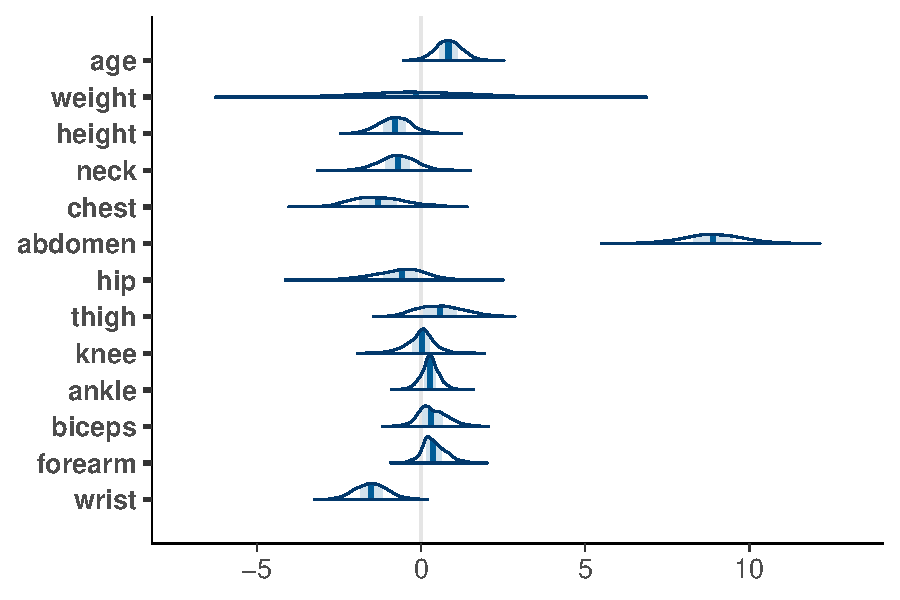
\includegraphics[width=10cm]{bodyfat_mcmc_areas.pdf}

\end{frame}

\begin{frame}
  
  {\Large\color{navyblue} Hypothesis testing and posterior dependencies}

  Looking at the marginal posterior(s) can be misleading when there
  are many parameters

  Bivariate marginal of weight and height
  
  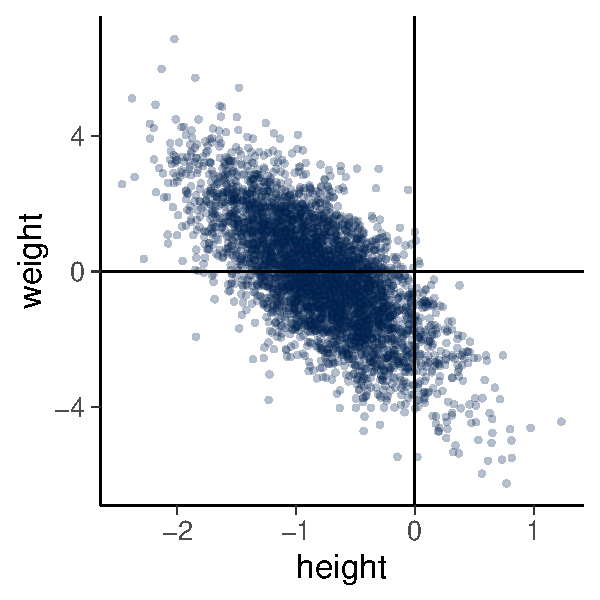
\includegraphics[width=7.5cm]{bodyfat_mcmc_scatter.pdf}

\end{frame}


\begin{frame}

  {\Large\color{navyblue} Hypothesis testing and posterior dependencies}

  In bodyfat example, starting from full model

  \begin{itemize}
  \item BF in favor of removing weight (p=0.92)
  \item LOO in favor of removing weight (p=0.99)
  \end{itemize}

  In bodyfat example, starting from model y $\sim$ abdomen
  \begin{itemize}
  \item BF in favor of adding weight (p=1.0)
  \item LOO in favor of adding weight (p=1.0)
  \end{itemize}

\end{frame}

\begin{frame}
  
  {\Large\color{navyblue} Variable selection}

  More elaborate approaches are needed for variable selection

  See Lecture 9.3 on projection predictive variable selection
  
  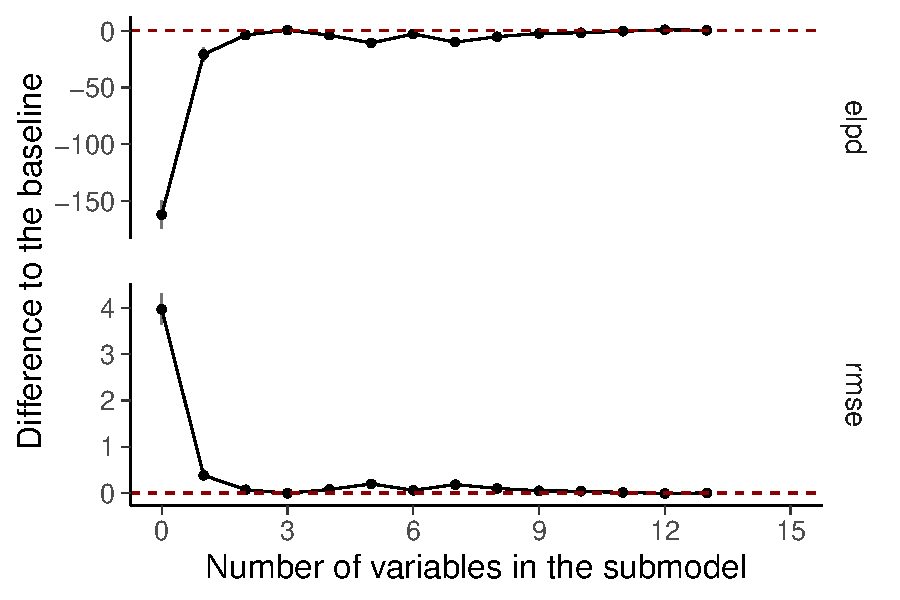
\includegraphics[width=10.5cm]{bodyfat_varsel_plot.pdf}

\end{frame}


\begin{frame}

  {\Large\color{navyblue} Common statistical tests as Bayesian models}

  Most common statistical tests are linear models
  
  {\small
  \begin{tabular}{lll}
   $t$-test & mean of data & {\tt stan\_glm(y \~\ 1)}\\
   paired $t$-test & mean of diffs &{\tt stan\_glm((y1 - y2) \~\  1)}\\
   Pearson correl. & linear model &{\tt stan\_glm(y \~\  1 + x)}\\
   two-sample $t$-test & group means &{\tt stan\_glm(y \~\  1 + gid)}\\
   ANOVA & hier. model &{\tt stan\_glm(y \~\  1 + (1 | gid))}\\
    $\ldots$ &
  \end{tabular}

  \uncover<2->{
  possible to extend, e.g., with group specific variances and and
  different distributions such $t$- or Poisson distribution}
}

  \uncover<3->{
  See longer list and illustrations (with {\tt lm}) at
  \url{https://lindeloev.github.io/tests-as-linear/}\\
  and\\
  in the forthcoming {\it Regression and other stories} book
  }

\end{frame}

\begin{frame}
  
  {\large\color{navyblue} Chapter 8: Modelling accounting for data collection}

  Highly recommended to read. Very informative, but also dense chapter.
  
  \begin{itemize}
  \item We need to model the data collection unless it is ignorable
  \item We need to know when data collection is ignorable
  \item<2-> Data collection
    \begin{itemize}
    \item Sample surveys
    \item Designed experiments
    \item Randomization
    \item Observational studies
    \item Censoring and truncation
    \end{itemize}
  \end{itemize}
  
\end{frame}

\begin{frame}
  
  {\large\color{navyblue} Chapter 14: Introduction to regression models}

  \begin{itemize}
  \item Justification of conditional modeling
    \begin{itemize}
    \item if joint model factorizes $p(y,x|\theta,\phi)={\color{blue}p(y|x,\theta)}(x|\phi)$\\
      we can model just ${\color{blue}p(y|x,\theta)}$
    \end{itemize}
  \item<2-> Gaussian linear model with conjugate prior
    \begin{itemize}
    \item the conditional posterior is multivariate normal
    \item with fixed prior on weights, the joint posterior is N-Inv-$\chi^2$
    \item<3-> these properties are sometimes useful and thus good to know,
      but with probabilistic programming less often needed
    \end{itemize}
  \item<4-> Bit on causal analysis (see much more in ROS)
  \item<5-> Assembling matrix of explanatory variables
    \begin{itemize}
    \item identifiability, collinearity, nonlinear relations,
      indicator and categorical variables, interactions
    \item variable selection is not much discussed (see lectures 9.2,9.3)
    \end{itemize}
  \item<6-> Regularization
    \begin{itemize}
    \item not much discussed (see more in lecture 9.3 and e.g. \url{https://betanalpha.github.io/assets/case_studies/bayes_sparse_regression.html})
    \end{itemize}
  \item<7-> Unequal variances and correlations
  \end{itemize}
  
\end{frame}

\begin{frame}
  
  {\large\color{navyblue} Lasso and Bayesian lasso}

  \begin{itemize}
  \item Lasso is penalized maximum likelihood linear regression, with
    L1 one penalty where the amount penalty is adapted
    \begin{itemize}
    \item<2-> penalized maximum likelihood finds the mode given the
      penalty parameter, and is almost the same as maximum a
      posteriori
    \item<3-> when the amount of penalty is increased, marginal modes of
      weak effects go to zero first
    \item<4-> when the amount of penalty is increased, also the relevant
      coefficients are shrunk towards zero
    \item<5-> sometimes relaxed lasso is used, where after variable
      selection coefficients are re-estimated
    \end{itemize}
  \item<6-> Bayesian lasso uses Laplace distribution as prior
    \begin{itemize}
    \item Laplace prior is equivalent to L1 penalty
    \item<7-> but the Bayesian inference includes distribution for
      parameters and that distribution doesn't shrink to a point at
      zero, even if the mode would be at zero
    \item<8-> empirically better results obtained with more
      sparse priors
    \item<9-> it's best to separate selection of sensible prior, good
      posterior inference, and the decision analysis of which
      variables are important
    \end{itemize}
  \end{itemize}
  
\end{frame}

\frame{

  {\Large\color{navyblue} Sparse priors}

  \includegraphics[width=6cm]{kappas.png}\\
  from Carvalho, Polson, Scott (2009).

}
\frame{

  {\Large\color{navyblue} Regularized horseshoe}

  \vspace{-0.5\baselineskip}
  \includegraphics[width=6.5cm]{hs_vs_spikeandslab.png}\\
  \includegraphics[width=6.5cm]{rhs_vs_spikeandslab.png}

  \vspace{-0.5\baselineskip}
  for more see
  \vspace{-0.5\baselineskip}
  \begin{itemize}
  \item 
  {\small Piironen and Vehtari (2017). Sparsity information and
      regularization in the horseshoe and other shrinkage priors. In
      Electronic Journal of Statistics, 11(2):5018-5051. \href{https://projecteuclid.org/euclid.ejs/1513306866}{Online}}
  \item  \url{https://betanalpha.github.io/assets/case_studies/bayes_sparse_regression.html}
  \end{itemize}
  

}

\frame{

  {\Large\color{navyblue} Projpred selection vs. Lasso}

  See projpred in lecture 9.3
  
Same simulated regression data as in lecture 9,3, \\�
$n=50$, $p=500$, $p_\text{rel} = 150$, $\rho=0.5$

\vspace{0.5em}

  \makebox[12.1cm][t]{
    \hspace{-0.5cm}
  \begin{minipage}{0.99\textwidth}
      \only<1>{\includegraphics[width=5.5cm]{vslasso1rmse.pdf}}
      \only<2>{\includegraphics[width=5.5cm]{vslasso2rmse.pdf}}
      \only<3->{\includegraphics[width=5.5cm]{vslasso3rmse.pdf}}
      \uncover<4>{\includegraphics[width=5.5cm]{vslasso3mlpd.pdf}}
  \end{minipage}
  }
  
}

\begin{frame}
  
  {\large\color{navyblue} Chapter 15: Hierarchical linear models}

  \begin{itemize}
  \item Since you know hierarchical models, theory is easy
  \item With probabilistic programming computation is also easy
    \begin{itemize}
    \item BDA3 discusses some other computational issues
    \item section on transformations for HMC is relevant\\ (see also
      Stan user guide 21.7 Reparameterization)
    \end{itemize}
  \item<2-> Fixed, random, and mixed effects models
    \begin{itemize}
    \item we don't recommend using these terms, but they are so
      popular that it's useful to know them
    \end{itemize}
    \uncover<3->{\hspace{-1cm}\small
        \begin{tabular}[t]{ll}
     {\tt y $\sim$ 1 + x} & fixed / population effect; pooled model\\
     {\tt y $\sim$ 1 + (0 + x | g) } & random / group effects \\
     {\tt y $\sim$ 1 + x + (1 + x | g) } & mixed effects; hierarchical model 
        \end{tabular}
      }
      \vspace{1\baselineskip}
  \item<3-> ANOVA in section 15.6 (see also {\tt stan\_aov})
  \end{itemize}
  
\end{frame}

\begin{frame}
  
  {\large\color{navyblue} Chapter 16: Generalized linear models}

  \begin{itemize}
  \item Bioassay model is an example of GLM
  \item<2-> Components:
    \begin{itemize}
    \item[1.] The linear predictor $\eta = X\beta$
    \item<3->[2.] The link function $g(\cdot)$ and $\mu = g^{-1}(\eta)$
    \item<4->[3.] Outcome distribution model with location parameter $\mu$
      \begin{itemize}
      \item<5-> the distribution can also depend on dispersion
        parameter $\phi$
      \item<6-> originally just exponential family distributions
        (e.g. Poisson, binomial, negative-binomial), which all have
        natural location-dispersion parameterization
      \item<7-> after MCMC made computation easy, GLM can refer to
        models where outcome distribution is not part of exponential
        family and dispersion parameter may have its own latent linear
        predictor
      \end{itemize}
    \item<8-> Hierarchical GLM natural extension
    \item<9-> 16.3 Weakly informative priors section is excellent
      although the recommendation on using Cauchy has changed (see
      \url{https://github.com/stan-dev/stan/wiki/Prior-Choice-Recommendations})
      
    \end{itemize}
  \end{itemize}

  
\end{frame}

\begin{frame}
  
  {\large\color{navyblue} Chapter 17: Models for robust inference}

  \begin{itemize}
  \item For example\\
    \begin{tabular}[t]{lcl}\small
      normal & $\rightarrow$ & $t$-distribution\\
      Poisson & $\rightarrow$ & negative-binomial \\
      binomial & $\rightarrow$ & beta-binomial \\
      probit & $\rightarrow$ & logistic / robit 
    \end{tabular}
  \item<2-> Computation with MCMC easy
    \begin{itemize}
    \item posterior can be multimodal
    \item<3-> rstanarm doesn't have $t$-distribution for outcome, but brms
      has
    \end{itemize}
  \end{itemize}

  
\end{frame}

\begin{frame}
  
  {\large\color{navyblue} Chapter 18: Models for missing data}

  \begin{itemize}
  \item Extends the data collection modelling from Chapter 8
  \item Useful terms 
    \begin{itemize}
    \item<2-> Missing completely at random (MCAR)\\
      missingness does not depend on missing values or other observed
      values (including covariates)
    \item<3-> Missing at random (MAR)\\
      missingness does not depend on missing values but may depend on
      other observed values (including covariates)
    \item<4-> Missing not at random (MNAR)\\
      missingness depends on missing values
    \end{itemize}
  \item<5-> Multiple imputation
    \begin{itemize}
    \item[1.] make a model predicting missing data
    \item[2.] sample repeatedly from the missing data model to generate
      multiple imputed data sets
    \item[3.] make usual inference for each imputed data set
    \item[4.] combine results
    \end{itemize}
  \end{itemize}
  
\end{frame}

\begin{frame}
  
  {\large\color{navyblue} Chapter 21: Gaussian process models}

  \begin{itemize}
  \item Gaussian process is 
    \begin{itemize}
    \item infinite dimensional extension of normal distribution
    \item useful prior for non-linear functions
    \item for any finite number of variables, the marginal is
      multivariate normal
    $f_1,\ldots,f_n  \sim \N\left(\mu( x_1,\ldots, x_n), K(x_1,\ldots,x_n) \right)$
    \end{itemize}
  \item<2-> Often a priori $\mu = 0$
  \item<3-> Prior for smooth non-linear functions, e.g. with\\
      $k(x,x') = \tau^2 \exp\left(-\,\frac{| x - x' |^2}{2l^2}\right)$
  \end{itemize}
  \vspace{-1\baselineskip}
 \only<4>{\hspace{-0.5cm}\includegraphics[width=12cm]{gpprior-eps-converted-to.pdf}}
 \only<5>{\hspace{-0.5cm}\includegraphics[width=12cm]{gpposterior-eps-converted-to.pdf}}
  
\end{frame}

\begin{frame}
  
  {\large\color{navyblue} Chapter 21: Gaussian process models}

  \begin{itemize}
  \item Conditional on covariance function parameter the posterior is
    just multivariate normal
    \begin{itemize}
    \item need to make inference for covariance function parameters
      given the marginal likelihood
    \item the exact computation of the marginal likelihood scales
      $O(N^3)$
    \end{itemize}
  \end{itemize}
  
\end{frame}


\begin{frame}

  \vspace{-0.85\baselineskip}
  \begin{itemize}
  \small
  \item Easy to make additive models\\
    $y_t(t) = f_1(t) + f_2(t) + f_3(t) + f_4(t) + f_5(t) +\epsilon_t$\\
    \includegraphics[width=7.5cm]{birthsnewbw-eps-converted-to.pdf}
  \end{itemize}  

\end{frame}

\begin{frame}
  
  {\large\color{navyblue} Chapter 21: Gaussian process models}

  \begin{itemize}
  \item For non-Gaussian outcome models similar extension as GLMs
  \item Survival model example:
  \end{itemize}

  \includegraphics[width=8cm]{gp_leukemia-eps-converted-to.pdf}
  
\end{frame}

\begin{frame}
  
  {\large\color{navyblue} GPs in Stan}

  \begin{itemize}
  \item GP specific software (e.g. GPy, GPflow, GPyTorch) scale
    computationally better for GPs than Stan
  \item Stan has some built-in covariance functions (and soon GPU support)
  \item In case of non-Gaussian outcome models, sampling of latent
    variables can be slow (Laplace integration over the latents coming)
  \item<2-> Instead of covariance matrix based approach, for low
    dimensional cases faster to use basis function representation
    \begin{itemize}
    \item e.g. {\tt stan\_glm(y $\sim$ s(x, bs="gp"))}
    \end{itemize}
  \end{itemize}

  
\end{frame}

\end{document}

%%% Local Variables: 
%%% TeX-PDF-mode: t
%%% TeX-master: t
%%% End: 
